%
%  analysis_report
%
%  Created by Sam Cook on 2012-11-06.
%  Copyright (c) 2012 . All rights reserved.
%
\documentclass[]{article}

% Setup for fullpage use
\usepackage{fullpage}

% More symbols
\usepackage{amsmath}
% even more symbols (mainly the lesssim)
% NB! usepackage is case sensitive
\usepackage{MnSymbol}

% Allow merged rows/colums in tables
\usepackage{multirow}
% Allow footnotes on tables
\usepackage{threeparttable}

% Package for including code in the document
\usepackage{minted}

% If you want to generate a toc for each chapter (use with book)
\usepackage{minitoc}

% This is now the recommended way for checking for PDFLaTeX:
\usepackage{ifpdf}

\ifpdf
\usepackage[pdftex]{graphicx}
\else
\usepackage{graphicx}
\fi

% useful commands for setting nth's (e.g. 5th) and alt versions (e.g. 2nd)
\newcommand{\nth}[1]{$#1^\text{th}$}
\newcommand{\nthTwo}[2]{$#1^\text{#2}$}
% quick macro for µs
\newcommand{\ms}{$~\mu$s}

\title{MuSIC 5 Analysis Report}
\author{Sam Cook}

\date{2012-11-06}

\begin{document}

\ifpdf
\DeclareGraphicsExtensions{.pdf, .jpg, .tif}
\else
\DeclareGraphicsExtensions{.eps, .jpg}
\fi

\maketitle


\begin{abstract}
    The \nth{5} MuSIC beam-time (\nth{18} to the \nthTwo{22}{nd} June 2012) was intended to test the momentum distribution of the muons beam. Here we will discuss the strategy employed to analyse the data and the problems encountered.
\end{abstract}

\section{Introduction} % (fold)
\label{sec:introduction}
The analysis of the \nth{5}~MuSIC beam time splits into 5~logical stages called here: `Run Data' (Section~\ref{sec:run_data}), `Simulated Data' (Section~\ref{sec:simulated_data}), `Secondary Calculations' (Section~\ref{sec:secondary_calculations}), `Fitting and Integration' (Section~\ref{sec:fitting_and_integration}) and `Muon Yield' (Section~\ref{sec:muon_yield}). The `Run' and `Simulated Data' algorithms cover the processing of the initial data to such a point as they can be treated identically. The `Secondary Calculations' section covers the calculation of the detector acceptance and dead time. The `Fitting and Integration' and `Muon Yield' sections cover the final stages of the algorithm in calculating the number of muon decays and ultimately the muon yield of the run. The overall flow can be seen in Figure~\ref{fig:analysis_flow_diagrm}. A brief overview of the experimental set up is given in section~\ref{sec:experimental_set_up}.

\begin{figure}[htbp]
    \centering
        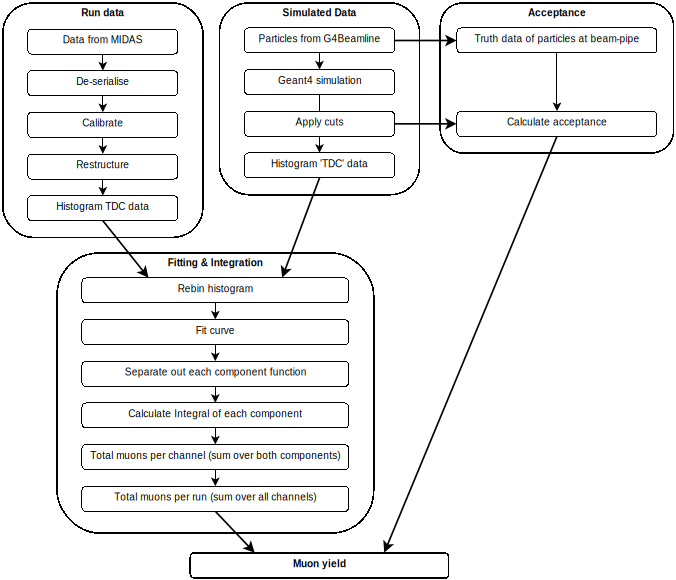
\includegraphics[height=0.49\textheight]{image/Analysis_flow_diagram.png}
    \caption{Flow diagram of the analysis' logic}
    \label{fig:analysis_flow_diagrm}
\end{figure}
% section introduction (end)
%%%%%%%%%%%%%%%%%%%%%%%%%%%%%%%%%%%%%%%%%%%%%%%%%%%%%%%%%%%%%%%%%%%%%%%%%%%%%%
\section{Experimental Set Up} % (fold)
\label{sec:experimental_set_up}
To measure the momentum distribution of the muon beam two separate problems had to be solved: firstly how to count the muons produced and secondly how to determine their momentum. The first problem is addressed by looking for muon decays through timing data whilst the second is dealt with by using degraders and a thin stopping target to select specific momentums. 

\subsection{Detector} % (fold)
\label{sub:detector}
The detector consisted of an aluminium degrader who's thickness could be varied to select different momentum ranges, a thin (1~mm) upstream counter and a thicker (3.5~mm) downstream counter on either side of a 0.5~mm copper stopping target. A schematic of the detector can be seen in figure~\ref{fig:setup}. Based on simulation (section~\ref{sec:simulated_data}) we can predict the mean momentum of muons that decay for different degrader thicknesses, the momentum distributions can be seen in figure~\ref{fig:stopped_muon_mom} with the mean momentums given in table~\ref{tab:stopped_muon_mom}.
\begin{figure}[htbp]
    \centering
        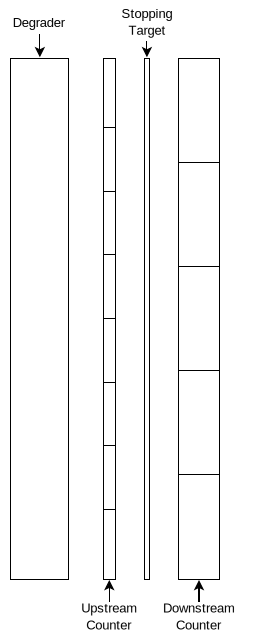
\includegraphics[scale=0.5]{image/Detector_setup.png}
    \caption{Experimental set up of the detector for MuSIC~5 (not to scale)}
    \label{fig:setup}
\end{figure}  
\begin{figure}[htbp]
    \centering
        \includegraphics[width=\textwidth]{image/stopped_muon_momentum.png}
    \caption{Simulated momentum distributions for muons decaying between the up and downstream counters. 900~M initial protons were simulated with a range of aluminium degrader thicknesses.}
    \label{fig:stopped_muon_mom}
\end{figure}
\begin{table}
    \begin{center}
    \begin{tabular}{r|r@{ $\pm$ }l|r@{ $\pm$ }l} % r@{ $\pm$ }l should align on \pm
        Degrader (mm) & \multicolumn{2}{|c|}{Mean (MeV/c)} & \multicolumn{2}{|c}{RMS (MeV/c)}\\
        \hline
        Air 5.0       & 41.03 & 0.21 & 21.59 & 0.15 \\
        Aluminium 0.5 & 46.68 & 0.20 & 19.84 & 0.14 \\
        Aluminium 1.0 & 50.29 & 0.21 & 19.13 & 0.15 \\
        Aluminium 5.0 & 65.66 & 0.22 & 16.86 & 0.16 \\
    \end{tabular}
    \end{center}
    \caption{Simulated mean momentums for decaying muons. 900~M initial protons}
    \label{tab:stopped_muon_mom}
\end{table}

The counters used were mylar wrapped scintillators with read-out performed by MPPCs mounted on either end of a wave length shifting fibre bounded along the long axis of the scintillator using optical cement. The signals from each pair of MPPCs are combined and amplified before being passed to the data acquisition system (DAQ) for processing.

% subsection detector (end)
\subsection{Data Acquisition} % (fold)
\label{sub:data_acquisition}
The Data Acquisition (DAQ) took two measurements: the time at which signals arrived from the MPPC and the strength of those signals. The timing measurements are of the primary concern for this analysis. The DAQ itself had 3 distinct stages: discrimination, trigger formation and readout.

MPPCs are inherently noisy devices and discrimination is required to separate signal due to scintillation events from the MPPC's noise. A voltage threshold was set which (when exceeded) created a digital signal. Two thresholds were used: a lower one for the upstream counter and a higher one for the downstream counter. The lower threshold for the, thinner, upstream counters enabled better detection of minimally ionising muons whilst the higher downstream threshold enabled better detection of the more ionising electrons produced by muon decay. 

Using the signals from the discriminator a trigger was created based on the signature of muonic decay: the anti-coincidence of the up and downstream counters. It was assumed that a muon that doesn't decay in the detector region will be seen in both counters within a very small window of time ($<$50~ns). The only other constraint on the formation of a trigger was that the system wasn't busy in which case the trigger couldn't be accepted.

The trigger, once formed, signalled the start of readout. There were 3 modules to be read out via VMEbus (VME): a charge to Digital Converter (QDC), a scaler and a Multi-hit Time to Digital Converter (MTDC) which is of primary concern for this analysis. The MTDC recorded all signals  within a 20\ms{} period following the trigger that passed discrimination and that were anti-coincident with the other counter. Using a MTDC ensured that even if some beam remnant or dark event created a signal then the real signal would also be recorded and determined with background removal. The channel assignment used for the MTDC can be seen in table~\ref{tab:mtdc_ch}. To increase the accuracy of the MTDC the trigger time is recorded on a seperate channel called `TDC0'.
\begin{table}
    \begin{center}
    \begin{tabular}{c|c|c}
        Channel & Signal & Notes\\
        \hline
        0  & TDC0 & Time at which the trigger was formed \\
        \hline
        1  & U1   & \multirow{8}{*}{Upstream Counter}\\
        2  & U2   & \\
        3  & U3   & \\
        4  & U4   & \\
        5  & U5   & \\
        6  & U6   & \\
        7  & U7   & \\
        8  & U8   & \\
        \hline
        9  & D1   & \multirow{5}{*}{Downstream counter}\\
        10 & D2   & \\
        11 & D3   & \\
        12 & D4   & \\
        13 & D5   & \\
        \hline
        14 & Ge1  & \multirow{2}{*}{Germanium counter (not used in this analysis)}\\
        15 & Ge2  & \\
    \end{tabular}
    \end{center}
    \caption{Channel assignment for the MTDC. QDC channel assignment follows the same scheme but has no entry for channel 0 (as TDC 0 will be one of the upstream counters by design).}
    \label{tab:mtdc_ch}
\end{table}

The scaler was used to record system diagnostics (e.g. the trigger rate) by polling the scaler regularly during each run. The QDC recorded the strength of the trigging signal by integrating its charge over 100~ns. This information has not be incorporated into the current analysis but may be used in later analysis, for example to apply more stringent energy cuts at trigger time or for selection of regions of interest. The QDC had the same channel assignment as the TDC but without the germanium detector (as it had its own analogue to digital converter) and TDC0 (which was a digital signal).
\begin{table}
    \centering
    \begin{tabular}{c|c|l}
        Channel & Signal & Notes\\
        \hline
        0 & SEC & Measure of the proton current\\
        1 & Trigger & number of t0's\\
        2 & U and $\overline{\text{D}}$ & count of potential triggers\\
        3 & U & Upstream only\\
        4 & D & Downstream only\\
        5 & Scint & -\\
        6 & unused & -\\
        7 & clk & Record of time passed\\
    \end{tabular}
    \caption{Table of scaler channels and their designation}
    \label{tab:scaler_chs}
\end{table}

% subsection data_acquisition (end)
% section experimental_set_up (end)
%%%%%%%%%%%%%%%%%%%%%%%%%%%%%%%%%%%%%%%%%%%%%%%%%%%%%%%%%%%%%%%%%%%%%%%%%%%%%%
\section{Run Data} % (fold)
\label{sec:run_data}
As figure~\ref{fig:analysis_flow_diagrm} shows there are 5 stages in preparing the experimental data for analysis (receipt of the data from MIDAS, de-serialisation, calibration, restructuring and histogramming). These will will be explained in more detail in the following sub-sections but the general process will be discussed here. The first stage is the receipt of data from the DAQ via MIDAS, this creates files of raw data which has to be de-serialised in the next stage before having calibration applied to it. The final stages are to restructure the data according to channel and then create histograms of the TDC values ready for analysis. 

These processes are split across 4 programs: MIDAS; mu\_analysis and mid2root\_converter (which act on .root and .mid MIDAS files respectively); and finally tdc\_file.py which is a python script for creating the TDC histograms.

\subsection{Data from MIDAS} % (fold)
\label{sub:data_from_midas}
MIDAS is `a general purpose data acquisition system for small and medium scale experiments'~\cite{ritt2012midas} and is the primary interface to the DAQ via VME. 

MIDAS stored the raw data from each run as a single file either in its own binary xml format (.mid files) or in ROOT~\cite{Brun199781} format (.root). Data was read from the VME crate in two asynchronous modes: `Trigger' and `Scaler' each corresponded to a separate tree structure in the resulting file. The majority of the time the system operated in trigger-mode: whenever a trigger was formed the controlling PC was informed and once the data had been gathered readout of the MTDC and QDC occurred via the VME. Scaler mode occurred at regular intervals and consisted of reading the diagnostics data gathered by the scaler, this did not reset the module which continued to accumulate data. 

Each tree contained a branch per module being read, the trigger tree also had also branch for errors (named `ERR'). The branches all had the same structure: an integer that recorded the number of values read and an array of integers containing those values. For the scaler and QDC modules the number of values read out was the same for every trigger as both had a fixed number of channels and took one measurement on each. The MTDC had a variable number of values to read out as it could record multiple hits on each channel.
% subsubsection data_from_midas (end)
\subsection{De-Serialisation} % (fold)
\label{sub:de_serialisation}
The first raw data from MIDAS for the MTDC and QDC were serialised and mangled with the channel number this means that they require processing before the real values can be extracted. Below are brief summaries of the algorithms used to de-serialise the MTDC data (listing~\ref{lst:mtdc_algo}), for full listings, including de-serialisation methods for QDC, see appendix~\ref{app:deserialisation}.
%
\begin{listing}[htbp]
    \begin{minted}[gobble=4]{c++}
    tdc_value      =  raw_val & 0x001f ffff
    tdc_channel    = (raw_val & 0x03e0 0000) >> 21
    tdc_valid_read = (raw_val & 0xf800 0000) == 0x0
    \end{minted}
    \caption{Method for de-serialising CAEN V1290N~\cite{CAENV1290N} data}
    \label{lst:mtdc_algo}
\end{listing}
% subsection de_serialisation (end)
\subsection{Calibration} % (fold)
\label{sub:calibration}
The MTDC has a stated least significant bit resolution of $\sim$25~ps with a 21 bits of data per value, this gives a maximum value of 52\ms{}. Conversion from the stored value to real, trigger aligned, time is done using the formula:
\begin{align}\label{equ:tdc_calibration}
    t'   &= \frac{1.025}{40}(t - TDC0)
\end{align}
where $t'$ is the calibrated time, $t$ is the de-serialised MTDC value and $TDC0$ is the de-serialised trigger time. The fraction is the number of MTDC bins per ns.
% subsection calibration (end)
\subsection{Restructure} % (fold)
\label{sub:restructure}
In order for the MIDAS data to be easily manipulated it was restructured. The initial format was a simple structure of one branch for each module (i.e. one for MTDC one for the QDC and a final one for errors). A second tree was used to store the scaler values. Each branch had a leaf for the number of values and a leaf with the array of values.

In the restructured file each channel is a branch of a tree with the following leaves: QDC, TDC0, nHITS, TDC[nHITS]. The QDC value is self-explanatory, TDC0 was the trigger time, nHITS was the number of entries recorded by the MTDC for that channel and TDC was an array of the values. The error data was ignored as was the scaler tree as these can be read from the original file if needed and neither was required for de-serialisation or calibration.
% subsection restructure (end)
\subsection{Histogramming} % (fold)
\label{sub:Histogramming}
Once the data has been restructured it is trivial to create a histogram of the TDC data for each channel which forms the basis of the later analysis. A basic bin width of 1~ns was used and a range from 0 to 20\ms. A time of 0 was used for the lowest bin as, although the data window began at 50~ns, the MTDC recorded data as a sliding window so some values prior to the trigger were also recorded. All the histograms for (i.e. for all channels for all runs) were saved in the same root file.
% subsection histogramming (end)
% section run_data (end)
%%%%%%%%%%%%%%%%%%%%%%%%%%%%%%%%%%%%%%%%%%%%%%%%%%%%%%%%%%%%%%%%%%%%%%%%%%%%%%
\section{Simulated Data} % (fold)
\label{sec:simulated_data}
To save simulation time and ensure accuracy three separate programs were created to simulate the beamline: the initial protons and beam transport system were simulated in G4Beamline~\cite{G4BL} (G4BL); the detector was simulated in a custom program implemented with Geant4~\cite{Agostinelli2003250}; and the digitisation and histogramming were done in ROOT.

\subsection{G4Beamline Particle Production} % (fold)
\label{sub:g4bl_particle_production}
Simulation of the bulk of the beamline (the pion capture solenoid and muon transport system) was done using a G4BL macro. G4BL is built using G4 and is designed to simplify the process of developing a simulation, in this way it has many of the strengths of G4 without the development time although because of this it doesn't have quiet the same flexibility. 900~million\footnote{ Geant4 and G4BL the same pseudo-random number generator, which guarantees a unique set of pseudo-random numbers for the first 900~million integer seeds, this means that for each particle simulated up to this value the pattern of random numbers generated is unique.} initial protons were simulated to be used as input to the Geant4 simulation. The protons were simulated interacting with the graphite target in the pion capture solenoid and then the resultant particles were transported to the end of the beam-pipe where a monitor recorded the distribution as a ROOT file for later use. 

Using a single simulation for the majority of the beam meant that the same particle distribution could be used for a variety of experimental configurations whilst avoiding long run times.

% subsection g4bl_particle_production (end)
\subsection{Geant4 Detector Simulation} % (fold)
\label{sub:geant4_detector_simulation}
As G4BL `does not simulate the performance of real-world detectors'~\cite{G4BL} a custom simulation was written using the Geant4 framework. This simulated the detector as 4 discrete volumes: the degrader, the stopping target and the two counters all embedded within a single world volume. The particle distribution from G4BL was used as primary particles. The magnetic field was simulated using the field-map supplied by Toshiba.

The simulation allowed variation of the degrader and stopping target material as well as their thickness. The width and height of the counters, stopping target and degrader were set to match those used in the real experiment. The counters were simulated as 2 large scintillators rather than individual strips for the sake of simplicity. For full listing on the simulation of the geometry see appendix~\ref{appsub:detector_geometry}.

Readout from the simulation was done by overloading the default SteppingAction. The SteppingAction is called for every step in a particles's track once all processes in that step have finished. It was overloaded so that if the particle was found to be within one of the 4 volumes then details of the particle would be recorded (see appendix~\ref{appsub:stepping_action} for the function use). Results were recorded in root files along with a copy of the primary particle information from G4BL. 

Control of the simulation was exerted using macros and command line arguments. The macros for a set of simulations (e.g. simulating the 4 degraders used in the experiment) were generated via bash scripts that made the set the appropriate flags as well as calling the simulation with the correct arguments.
% subsection geant4_detector_simulation (end)
\subsection{Digitisation \& histogramming} % (fold)
\label{sub:digitisation_histogramming}
Once the detector simulation was complete the data from it had to be ``digitised'' and histogrammed (the last two stages of the `simulated data' process) so as to be in the same format as the real data. This was done by making cuts on the data that mimicked those imposed by the DAQ. 

Using ROOT (`a data analysis framework'~\cite{Brun199781}) two cuts were applied to the simulated data. The first was that only charged particles could be selected (muons, electrons, pions and protons). The second cut applied was that the particle's parent had to have been seen in the upstream counter and it had to be seen in the downstream counter. 

Particles that passed the two cuts had the difference in their times at the up and downstream counters calculated and added to the output histogram. The entire digitisation macro can be found in appendix~\ref{appsub:digitisation_macro}. Unlike the real data only one histogram per `run' was created; all were saved to the same root file.
% subsection digitisation_histogramming (end)
% section simulated_data (end)
%%%%%%%%%%%%%%%%%%%%%%%%%%%%%%%%%%%%%%%%%%%%%%%%%%%%%%%%%%%%%%%%%%%%%%%%%%%%%%
\section{Secondary calculations} % (fold)
\label{sec:secondary_calculations}
There are two secondary calculations that need to be performed to calculate the muon yield. These are the acceptance, the fraction of the total beam we can expect to detect, and the dead time, a measure of how much of the time the detector is unable to process new data due to being busy.
\subsection{Acceptance} % (fold)
\label{sub:acceptance}
To calculate the acceptance the ratio of initial muons to muons that passed a `trigger' cut was calculated. This is done by counting the number of muons in simulated G4BL output (section~\ref{sub:g4bl_particle_production}) and then using a macro similar to that used to digitise the simulation output (section~\ref{sub:digitisation_histogramming}) to mimic the triggering process.

The main difference between the acceptance macro (appendix~\ref{app:acceptance}) and the digitisation macro (appendix~\ref{appsub:digitisation_macro}) were in the cuts applied to select the particles. Rather than any possible parent particle in the upstream detector only muons are selected, similarly, in the downstream detector only electrons who had a parent muon are selected.

The acceptance is then the ratio of muon/electron pairs to the initial number of muons:
\begin{align}
    \text{Acceptance} &= \frac{\text{Decay muons}}{\text{Initial Muons}} \label{equ:acceptance}
\end{align}
It is worth noting that given the above definition and method the acceptance changes due to the thickness and type of degrader used. Obviously a degrader that removed the majority of the muons from the beam will have a smaller acceptance as a smaller fraction of the beam will have survived to be detected. The results of the acceptance calculations are given in table~\ref{tab:acceptance}, the macro used can be seen in appendix~\ref{app:acceptance}.
\begin{table}
    \begin{center}
    \begin{tabular}{c| r@{ $\pm$ }l | r@{ $\pm$ }l | r@{ $\pm$ }l }
        Degrader (mm) & \multicolumn{2}{|c}{Decay Muons} & \multicolumn{2}{|c}{Initial Muons} & \multicolumn{2}{|c}{Acceptance (\%)}\\
        \hline
        Air 5.0       & 8089 & 90 & 95719 & 310 & 8.5 & 0.1 \\
        Aluminium 0.5 & 7068 & 84 & 95719 & 310 & 7.4 & 0.1 \\
        Aluminium 1.0 & 6394 & 80 & 95719 & 310 & 6.7 & 0.1 \\
        Aluminium 5.0 & 4180 & 65 & 95719 & 310 & 4.4 & 0.1 \\
    \end{tabular}
    \end{center}
    \caption{Table of the variance of acceptance with degrader thickness}
    \label{tab:acceptance}
\end{table}
% subsection acceptance (end)
\subsection{Dead time} % (fold)
\label{sub:dead_time}
The calculation of the dead time is unlike that of the acceptance as it was calculated based on the real data rather than simulation. Using the scaler it is possible to estimate how much of the time the DAQ was busy and hence what percentage of data was missed. 

As was stated in section~\ref{sub:data_acquisition} the scaler was used to record diagnostics on the DAQ. To calculate the dead time only two are needed, the trigger count and the potential trigger count which can be used to calculate the dead time thus:
\begin{align}
    D = \frac{\text{Potential Triggers}}{\text{Good Triggers}}
\end{align}
Where potential triggers are considered any anti-coincidence of the up without the downstream counter and a good trigger is one in which this occurs without the system being busy. The results for are given in table~\ref{tab:dead_time}.
\begin{table}
    \begin{center}
    \begin{tabular}{c|c|c|r@{ $\pm$ }l|r@{ $\pm$ }l|r@{ $\pm$ }l }
        Run & Degrader (mm of Al) & Run time (s) &
                              \multicolumn{2}{|c}{Good Triggers} &      
                              \multicolumn{2}{|c}{Potential Triggers} &
                              \multicolumn{2}{|c}{Dead time (\%)} \\
        \hline
        448 & 0.0 & 9221 & 9652965 & 3106 & 15678757 & 3959 & 61.6 & 11.3 \\
        451 & 0.5 & 1001 &  767321 & 875  &  1070366 & 1034 & 71.7 & 18.3 \\
        452 & 0.5 & 4944 & 3459886 & 1860 &  4667767 & 2160 & 74.1 & 15.7 \\
        455 & 1.0 & 6307 & 4090246 & 2022 &  5372409 & 2317 & 76.1 & 15.8 \\
        458 & 5.0 & 5144 & 2049077 & 1431 &  2454952 & 1566 & 83.5 & 19.0 \\
        459 & 5.0 & 2452 &  915314 & 956  &  1077534 & 1038 & 84.9 & 21.4 \\
    \end{tabular}
    \end{center}
    \caption{Dead time for each run along with the number of potential and good triggers. Run time is included to show the origin of the different counts.}
    \label{tab:dead_time}
\end{table}

% subsection dead_time (end)
% section secondary_calculations (end)
%%%%%%%%%%%%%%%%%%%%%%%%%%%%%%%%%%%%%%%%%%%%%%%%%%%%%%%%%%%%%%%%%%%%%%%%%%%%%%
\section{Fitting And Integration} % (fold)
\label{sec:fitting_and_integration}
This section won't follow the figure~\ref{fig:analysis_flow_diagrm} stages too closely as they are heavily entwined, instead the algorithm will be broken into two sections: the theory (section~\ref{sub:the_theory}) and the implementation (section~\ref{sub:the_implementation}).

\subsection{The theory} % (fold)
\label{sub:the_theory}
Once both the real and simulated data has been processed and put into histograms they can be treated identically. In order measure the number of decays the histograms are fitted with the function 
\begin{align}
    P(signal) &= N_{b} + N_{f}e^{-t / \tau_{f}} + N_{c} e^{-t / \tau_{c}} \label{equ:fit}
\end{align}
Where $N_{b}$ is a flat modelling of the background; $N_{f}$ and $\tau_{f}$ are the contribution of the free muon part and the free muon lifetime respectively; and $N_{c}$ and $\tau_{c}$ are the muonic-copper contribution and lifetime. Once the histogram has been fitted with equation~\ref{equ:fit} integrating either exponential portion of it and dividing by the bin width gives the number of muon decays corresponding to that mode. Similarly the total number of muons is given by the sum of the two integrals:
\begin{align}
    N_{\mu} &= \frac{1}{B} \int_{l}^{u}\left(N_{f}e^{-t / \tau_{f}} + N_{c} e^{-t / \tau_{c}} \right) \label{equ:sum_exp_parts}
\end{align}
where $N_{\mu}$ is the total number of muon decays in the histogram and $l$ and $u$ are the lower and upper bounds of the fit respectively. 

% subsection the_theory (end)
\subsection{The implementation} % (fold)
\label{sub:the_implementation}
The implementation of the above algorithm is done using pyROOT~\cite{lavrijsenpyroot} which is a python wrapper for ROOT~\cite{Brun199781}. Python is a preferable language to C++ for complex analysis as it is generally less verbose (allowing more rapid development and fewer bugs) as well as incorporating more powerful data structures (such as dictionaries) into the core language. Being a loosely typed language python can handle mixed-type objects which means that all the data for run can be kept in a single structure. For concrete listings of each stage from figure~\ref{fig:analysis_flow_diagrm} see appendix

There are 8 parameters that need to be set before the fit can proceed these are show in table~\ref{tab:typical_fit_values} with typical initial values. These fall into two broad groups: `fit settings' which relate to the bounds on the fitting method and the `initial parameter values' which determine what values the fit uses as start points for its approximations. The fit settings primarily affect how good a fit is achieved whilst the initial parameter values are mainly chosen to ensure that there are no degeneracies in the fit. 

\begin{table}
    \begin{center}
	    \begin{threeparttable}
		    \begin{tabular}{c | c | c }
		        Type & Parameter   & Value \\
		        \hline
		        \multirow{3}{*}{Fit Settings} & Bin width   & 75~ns \\
		                                      & Lower bound & 50~ns \\
		                                      & Upper bound & 20\ms \\
		        \hline
		        \multirow{3}{*}{Initial fit parameters} 
		                    & $N_{b}$     & $^1/_{10} \times$ maximum bin value \\
		                    & $N_{c}$     & Maximum bin value\\
		                    & $N_{f}$     & $^1/_{2} \times$ maximum bin value\\
		                    & $\tau_{c}$  & 163.5~ns $\pm$ 1~ns\\
		                    & $\tau_{f}$  & $\sim$2\ms\tnote{a}\\
		    \end{tabular}
		    \caption{Typical values for the fit parameters. \textbf{NB} that the copper value is often constrained as it is well know, the free muon lifetime is not well known as it is dependant on the combination of the muon lifetime in air, scintillator and as a free particle.}
		    \begin{tablenotes}
		        \item [a] The canonical free muon lifetime is 2.1969811$\pm$0.0000022\ms~\cite{Beringer2012}, see text for why this value is not fixed.
		    \end{tablenotes}
		    \label{tab:typical_fit_values}
	    \end{threeparttable}
    \end{center}
\end{table}

The largest changes to the fit are due to the fit settings. These determine the range that is fitted and the smoothness of the data that the fit is attempted on. The lower bound of the range probably has the largest affect on the fit. It is obvious that a large enough lower bound will utterly remove the region in which the copper component is dominant, to avoid this the minimum value of 50~ns is usually chosen. The upper bound has very little affect for any reasonable value ($>$15\ms) as that portion of the histograms is usually flat. The bin width has an important part to play as it the prime method of smoothing data. This is especially important as there is apparently a source of high frequency noise ($\sim$16~MHz) this is suspected to be due to the cyclotron setting the bin width to larger than $\sim$60~ns removes the affect of this.

The initial fit parameters were set by `eyeball' to approximations of their expected value, if this were not done ROOT would set all values to 0. A reasonably large range of values was chosen to avoid degeneracies (this is especially important to make sure that each fit corresponds to its label). $\tau_{c}$ is generally fixed to a range of $\pm$1~ns about its canonical value of 163.5~\cite{PhysRevC.35.2212} as this is a known value reasonably different compared to the other muonic lifetimes\footnote{The lifetimes for the other major materials in the detector are: Hydrogen 2194.903$\pm$0.066, Carbon 2026.3$\pm$1.5~ns, Nitrogen 1906.8$\pm$3.0~ns, Oxygen 1795.4$\pm$2~ns~\cite{PhysRevC.35.2212}. Where the scintillator is assumed to be mostly carbon and hydrogen and the air mainly nitrogen and oxygen.}. It is worth noting that only the negatively charged muons can form muonic atoms and so the copper component of the fit makes a reasonable approximation to this number whilst the free component will be composed of positively and negatively charged muons.

Once the histograms were fitted the fit parameters were extracted and used to create sub-functions corresponding to the individual components. Using ROOT's `Integral' and `IntegralError' functions the number of decays for each channel corresponding to each component could then be calculated. Equally summing over all the channels in a run the total number of muons for that run could be calculated.
% subsection the_implementation (end)
% section fitting_and_integration (end)
%%%%%%%%%%%%%%%%%%%%%%%%%%%%%%%%%%%%%%%%%%%%%%%%%%%%%%%%%%%%%%%%%%%%%%%%%%%%%%
\section{Muon Yield} % (fold)
\label{sec:muon_yield}
Once the number of muons for each run is known the muon yield is ultimately a matter of scaling. The formula used is:
\begin{align}
    Y = \frac{N_{mu}}{\epsilon \times A \times D \times t_{r} \times I}
\end{align}
Where $Y$ is the yield, $N_{mu}$ the number of muons for that run, $\epsilon$ is the detector efficiency, $A$ the acceptance for that degrader thickness, $D$ is the dead-time, $t_{r}$ is the run time in seconds and $I$ is the proton current.
% TODO DEAD TIME!
% section muon_yield (end)
%%%%%%%%%%%%%%%%%%%%%%%%%%%%%%%%%%%%%%%%%%%%%%%%%%%%%%%%%%%%%%%%%%%%%%%%%%%%%%
\section{Conclusion} % (fold)
\label{sec:conclusion}
As can be seen from figure~\ref{fig:why_its_buggered} there is a large disagreement between data and simulation as to the muon yield. There seems to be no obvious source for this discrepancy. There are shortcomings in the analysis and simulation but none would be expected to account for such a difference. Obviously the next stage of the analysis is to work through these to ensure that they do not. 
\begin{figure}[htbp]
    \centering
        \includegraphics[width=\textwidth]{image/sim_vs_data.eps}
    \caption{Comparison of simulation and data. Simulation are the 4 points across the top, data along the bottom.}
    \label{fig:why_its_buggered}
\end{figure}

The most obvious deficiency in the analysis is the lack optical processes in the simulation. Implementing these processes would be the first obvious step in establishing the cause of the difference that we see. Another obvious weakness is the lack of a thorough testing regime to ensure correctness in the simulation, again, this will be high on the priority list to ensure that the simulation is acting as we expect. 

% section conclusion (end)
\pagebreak
%%%%%%%%%%%%%%%%%%%%%%%%%%%%%%%%%%%%%%%%%%%%%%%%%%%%%%%%%%%%%%%%%%%%%%%%%%%%%%
%       APPENDIX
%%%%%%%%%%%%%%%%%%%%%%%%%%%%%%%%%%%%%%%%%%%%%%%%%%%%%%%%%%%%%%%%%%%%%%%%%%%%%%
\appendix
\section{De-serialisation} % (fold)
\label{app:deserialisation}
%
These are listings of the functions used to de-serialise CAEN V1290N (MTDC)~\cite{CAENV1290N} and CAEN V792N (QDC)~\cite{CAENV792N} data. They are extracts from the `midus file' object, written in C++.
%
\begin{minted}[gobble=4, linenos=True, stepnumber=5, numberblanklines=False]{c++}
    // Functions used for de-serialising CAEN V1290N MTDC.
    inline int midus_file::get_tdc_val(const int index) const {
    // Mask the data to get the recorded value from the MTDC branch at index
        unsigned int const tdc_data_mask = 0x01fffff;
        unsigned int const val = static_cast<unsigned int>(branches_m[tdc_i].data[index]);
        return static_cast<int>(val & tdc_data_mask);
    }
    
    inline int midus_file::get_tdc_ch(const int index) const {
        unsigned int const tdc_channel_mask = 0x03e00000;
        unsigned int const val = static_cast<unsigned int>(branches_m[tdc_i].data[index]);
        return static_cast<int>((val & tdc_channel_mask) >> 21);
    }
    
    inline bool midus_file::is_good_tdc_measure(const int index) const {
    // This checks the error bits
        unsigned int const tdc_data_type_mask = 0xf8000000;
        unsigned int const tdc_measurement    = 0x00000000;
        unsigned int const val = static_cast<unsigned int>(branches_m[tdc_i].data[index]);
        return ((val & tdc_data_type_mask) == tdc_measurement);
    }
    
    // Functions used for de-serialising CAEN V792N QDC.
    inline int midus_file::get_qdc_val(int const index) const {
    // Mask the data to get the QDC value from the branch at index
        unsigned int const data_mask = 0x00000fff;
        unsigned int const val = static_cast<unsigned int>(branches_m[qdc_i].data[index]);
        return static_cast<int>(val & data_mask); 
    }
    
    inline int midus_file::get_qdc_ch(const int index) const {
        unsigned int const channel_mask = 0x001f0000;
        unsigned int const val = static_cast<unsigned int>( branches_m[qdc_i].data[index]);
        return static_cast<int>((val & channel_mask) >> 17);
    }
    
    
    
    
    inline bool midus_file::is_good_qdc_measure(const int index) const {
    // Check for over/under flow in the value
        unsigned int const underflow_mask = 0x00002000;
        unsigned int const overflow_mask  = 0x00001000;
        unsigned int const val = static_cast<unsigned int>(branches_m[tdc_i].data[index]);
        return !((underflow_mask & val) || (overflow_mask & val));
    }
\end{minted}
% section tdc_deserialisation (end)
%%%%%%%%%%%%%%%%%%%%%%%%%%%%%%%%%%%%%%%%%%%%%%%%%%%%%%%%%%%%%%%%%%%%%%%%%%%%%%
\section{Detector simulation} % (fold)
\label{app:detector_simulation}
\subsection{Detector Geometry} % (fold)
\label{appsub:detector_geometry}
The C++ code used in the Geant4 required `Detector Constructor'. It creates a series of volumes that represent the components of the detector. Each volume has a placement, physical geometry and material properties.
 
\begin{minted}[gobble=4, linenos=True, stepnumber=5, numberblanklines=False]{c++}
    void DetectorConstruction::DefineMaterials() {
        // Tell Geant4 which elements, compounds and mixtures are going to be used
        // and what their properties and definitions are. 
        
        G4String symbol;        
        G4double a, z, density, fractionmass; 
        G4int ncomponents, natoms;
        
        // Elements for use in compounds/mixtures
        G4Element* H  = new G4Element("Hydrogen",symbol="H" , z= 1., a= 1.01*g/mole);
        G4Element* C  = new G4Element("Carbon"  ,symbol="C" , z= 6., a= 12.01*g/mole);
        G4Element* N  = new G4Element("Nitrogen",symbol="N" , z= 7., a= 14.01*g/mole);
        G4Element* O  = new G4Element("Oxygen"  ,symbol="O" , z= 8., a= 16.00*g/mole);
        
        // elements that will be used on their own.
        Al = new G4Material("Aluminium", z=13.0, a= 26.98 *g/mole, density= 2.700*g/cm3);
        Pb = new G4Material("Lead",      z=82.0, a= 207.19*g/mole, density= 11.35*g/cm3);
        Mg = new G4Material("Magnesium", z=12.0, a= 24.305*g/mole, density= 1.738*g/cm3);
        Cu = new G4Material("Copper",    z=29.0, a= 63.546*g/mole, density= 8.94 *g/cm3);
    
        // mixtures and compounds
        // Scintillator, most likely Polyvinyltoluene. See pg322 of Mokhov (2001) for calculated stopping power
        Scint = new G4Material("Scintillator", density= 1.032*g/cm3, ncomponents=2);
        Scint->AddElement(C, natoms=9);
        Scint->AddElement(H, natoms=10);
        
        // Mylar, used for wrapping the scintillators
        Mylar = new G4Material("Mylar", density= 1.397*g/cm3, ncomponents=3);
        Mylar->AddElement(C, natoms=10);
        Mylar->AddElement(H, natoms= 8);
        Mylar->AddElement(O, natoms= 4);
    
        // The detectors weren't in vacuum
        Air = new G4Material("Air"  , density= 1.290*mg/cm3, ncomponents=2);
        Air->AddElement(N, fractionmass=0.7);
        Air->AddElement(O, fractionmass=0.3);
    
        // More plastics for comparison
        Polyethylene = new G4Material("Polyethylene",density= 0.94*g/cm3, ncomponents=2);
        Polyethylene -> AddElement(H,0.14);
        Polyethylene -> AddElement(C,0.86);
    
        Polystyrene = new G4Material("Polystyrene", density= 1.03*g/cm3, 2);
        Polystyrene->AddElement(C, 8);
        Polystyrene->AddElement(H, 8);
        
        // print table
        G4cout << *(G4Material::GetMaterialTable()) << G4endl;
    }
    
    G4ThreeVector get_global_pos(double dist_from_coil8) {
        // Convert from centralised co-ordinates to rotated co-ordinates matching 
        // the Toshiba field map.
        double coil8_x = (776.3)*mm;
        double coil8_z = (3420.1)*mm;
        double glb_x = dist_from_coil8*sin(36.0*deg) + coil8_x;
        double glb_z = dist_from_coil8*cos(36.0*deg) + coil8_z;
        return G4ThreeVector(glb_x,0.0,glb_z);
    }
    
    G4VPhysicalVolume* DetectorConstruction::Construct() {
    //-------------------------------------------------------------------------
       // Magnetic field
       //-------------------------------------------------------------------------
        if (f_myField) {
            // Reload the magnetic field map every time the detector is constructed
            delete f_myField;
        }
    
        if(!f_myField) {
        // make the field map as a combination of the dipole & solenoid fields
            f_myField = new Field(f_fname_sol,f_fname_dip,f_dip_polarity);
            G4FieldManager* fieldMgr
                    = G4TransportationManager::GetTransportationManager() ->GetFieldManager();
            fieldMgr->SetDetectorField(f_myField);
            fieldMgr->CreateChordFinder(f_myField);
        }
    
       //-------------------------------------------------------------------------
       // Rotation Matrix
       //-------------------------------------------------------------------------
        G4RotationMatrix rot_36 = G4RotationMatrix();
        rot_36.rotateY(36.0*deg);
    
    
       //-------------------------------------------------------------------------
        // Detector Geometry
       //-------------------------------------------------------------------------
       
        // The world volume: this is the outer most volume of the simulation
        // For simplicity make the world the size of the field maps
        double world_hx = (8000/2.0)*mm; 
        double world_hy = (8000/2.0)*mm;
        double world_hz = (8000/2.0)*mm;
        
        // Create the solid geometry (in this case a simple box)
        G4Box * solid_world = new G4Box("world",world_hx,world_hy,world_hz);
        
        // The `logical' volume: material, geometry, if it's a detector etc
        f_logic_world = new G4LogicalVolume(solid_world,   // geometry of the vol
                                            Air,           // volume's material
                                            "world",       // volume's name
                                            0,             // field manager ptr
                                            0,             // sensitive detector ptr
                                            0);            // user limits
        
        // Place the logical volume (in the world's case it's automatically at 
        // the origin with no rotation)
        f_physi_world = new G4PVPlacement(0,               // Rotation
                                          G4ThreeVector(), // Translation
                                          f_logic_world,   // Logical volume
                                          "world",         // Name
                                          0,               // Mother (always null for world)
                                          false,           // Not used
                                          0);              // Copy number of volume
    
        // offset of the upstream counter with respect to coil8 
        // of the transport solenoid
        double coil8_to_scint1 = 440*mm; 
        
        // Dimensions of both counters are the same in xy plane, only the 
        // thickness (z) changes
        double sci_hx = (450.0/2.0)*mm; 
        double sci_hy = (450.0/2.0)*mm;
        
        // Translate the upstream counter from the origin to the end of
        // the beam pipe
        G4ThreeVector sci1_pos = get_global_pos(coil8_to_scint1);
        
        // The solid for the upstream counter
        G4Box* solid_sci1 = new G4Box("sci1", sci_hx, sci_hy, f_scint1z/2.0);
        // The logical volume. The counter doesn't have an associated sensitive
        // detector as that is resolved in the SteppingAction
        f_logic_sci1 = new G4LogicalVolume(solid_sci1,f_scint1Mat,"sci1",0,0,0);
        // place and rotate the volume at the end of the beam pipe
        f_physi_sci1 = new G4PVPlacement(G4Transform3D(rot_36,sci1_pos), f_logic_sci1, 
                                         "sci1", f_logic_world,false,0);
    
        // Copper stopping target
        double target_posZ = coil8_to_scint1 + (f_scint1z/2.0) + 3 + (f_targetZ/2.0); // 3 is thickness of separators
        double target_hx = (450.0/2.0)*mm;
        double target_hy = (450.0/2.0)*mm;
        G4ThreeVector target_pos = get_global_pos(target_posZ);
        G4Box* solid_target = new G4Box("target",target_hx,target_hy,f_targetZ/2.0);
        f_logic_target = new G4LogicalVolume(solid_target,f_targetMat,"target",0,0,0);
        f_physi_target = new G4PVPlacement(G4Transform3D(rot_36,target_pos), f_logic_target, 
                                           "target", f_logic_world, f alse,0);
    
       // scintillator bar (sci2)
       // dimensions are the same as scint 1 (other than thickness)
        double scint2_posz = target_posZ + 3 + (f_scint2z/2.0);
        G4ThreeVector sci2_pos = get_global_pos(scint2_posz);
        G4Box* solid_sci2 = new G4Box("sci2", sci_hx, sci_hy, f_scint2z/2.0);
        f_logic_sci2 = new G4LogicalVolume(solid_sci2,f_scint2Mat,"sci2",0,0,0);
    
        f_physi_sci2 = new G4PVPlacement(G4Transform3D(rot_36,sci2_pos), f_logic_sci2,
                                         "sci2", f_logic_world,false,0);
    
        // degrader
        // degrader is in front of scint 1
        double degrader_posz = coil8_to_scint1 - (f_scint1z/2.0) - 3 - (f_degraderZ/2.0);
        double degrader_hx = (450.0/2.0)*mm;
        double degrader_hy = (450.0/2.0)*mm;
        G4ThreeVector degrader_pos = get_global_pos(degrader_posz);
        G4Box* solid_degrader = new G4Box("degrader",degrader_hx,degrader_hy,f_degraderZ/2.0);
        f_logic_degrader = new G4LogicalVolume(solid_degrader,f_degraderMat,"degrader",0,0,0);
        f_physi_degrader = new G4PVPlacement(G4Transform3D(rot_36, degrader_pos), f_logic_degrader,
                                             "degrader", f_logic_world, false,0);
    
        // Set the user limits; these set a maximum step length for particles depending 
        // on which volume they are in. In this case the distance is 0.1*z-extent
        double scint1_limit = 0.1 * f_scint1z; // calculate the lengths
        double scint2_limit = 0.1 * f_scint2z;
        double st_limit = 0.1 * f_targetZ;
        double deg_limit = 0.1 * f_degraderZ;
        
        // Set the limits for the upstream counter...
        f_scint1_limit = new G4UserLimits(scint1_limit);
        f_logic_sci1->SetUserLimits(f_scint1_limit);
        
        // ...the downstream counter...
        f_scint2_limit = new G4UserLimits(scint2_limit);
        f_logic_sci2->SetUserLimits(f_scint2_limit);
        
        // ... the stopping target ...
        f_st_limit = new G4UserLimits(st_limit);
        f_logic_target->SetUserLimits(f_st_limit);
    
        // ... and the degrader.
        f_deg_limit = new G4UserLimits(deg_limit);
        f_logic_degrader->SetUserLimits(f_deg_limit);
    
        // Return the world (and hence all its child volumes) to the run manager
        return f_physi_world;
    }
\end{minted}
% subsection detector_geometry (end)
\subsection{Stepping Action} % (fold)
\label{appsub:stepping_action}
G4 simulates particles by stepping them through the volumes of the detector. In each step it calculates the lengths over which various events can occur (e.g. decaying or passing into another volume) which ever event has the shortest length is carried out. For each step along the particle's trajectory a user defined action (`SteppingAction') is also performed. This is what is used to generate output from the simulation. If the particle is found to be within a volume of interest (i.e. a counter, the stopping target or degrader) its details are recorded.
\begin{minted}[gobble=4, linenos=True, stepnumber=5, numberblanklines=False]{c++}
    void SteppingAction::UserSteppingAction(const G4Step * aStep) {
        // Action to be performed every step.
        
        G4Track * track = aStep->GetTrack();
        
        // The start of the current step
        G4StepPoint* point1 = aStep->GetPreStepPoint();
        // The start of the next step
        G4StepPoint* point2 = aStep->GetPostStepPoint();
        
        // If either pre or post point is null the particle is likely leaving the 
        // world or in an error state
        if (point2==NULL || point1==NULL) return;
    
        // We want to be able to access information on where the particle is going and where it is
        const G4VPhysicalVolume* nextvol = point2->GetTouchableHandle()->GetVolume();
        const G4VPhysicalVolume* thisvol = point1->GetTouchableHandle()->GetVolume();
        
        // if there is no next volume we're exiting the world
        if (!nextvol) return;
        
        // If the first point of the next step is in a new volume then we're
        // leaving this one
        bool last_step  = (point2->GetStepStatus() == fGeomBoundary);
        // If the first point of this step is at a boundary we've just entered it
        bool first_step = (point1->GetStepStatus() == fGeomBoundary);
        // Find out where we are
        const G4String& volname = thisvol->GetName();
        
        // We want information on the particles before they interact with the detector
        // so we select those specially by selecting those leaving the world and
        // entering the degrader 
        bool entering_degrader = last_step &&
                                 (nextvol->GetName() == "degrader") &&
                                 (volname == "world");

        // Codify the volume names
        int acounter = 0; 
        if     ( volname == "sci1" )     { acounter = 1; } 
        else if( volname == "target" )   { acounter = 2; } 
        else if( volname == "sci2" )     { acounter = 3; }
        else if( volname == "degrader" ) { acounter = 4; }
        else if( entering_degrader )     { acounter = 5; }
        else return; // not in a volume we're interested in
        
        // Get all the information that we want to store:
        // The parent particle's track ID (0 if this is the primary particle)
        int parentid = track->GetParentID();
        // This particle's track ID
        int trkid = track->GetTrackID();
        // What sort of particle is this
        int pdgid  = track->GetDefinition()->GetPDGEncoding();
        // Ek
        double kinetic = track->GetKineticEnergy()/MeV;
        // How long since the primary particle was produced in simulation time
        double tof = track->GetGlobalTime()/ns;
        // Where is the particle
        double x = track->GetPosition().x()/mm;
        double y = track->GetPosition().y()/mm;
        double z = track->GetPosition().z()/mm;
        // What is it's momentum
        double px = track->GetMomentum().x()/MeV;
        double py = track->GetMomentum().y()/MeV;
        double pz = track->GetMomentum().z()/MeV;
        // Sum of energy lost due to continuous processes and energy lost due to
        // secondary particles that were not simulated due to being below the cut
        // threshold (i.e. not including secondaries actually simulated)
        double edep = aStep->GetTotalEnergyDeposit()/MeV;
        // Get the name of the process that is currently limiting the step length
        const G4String& procname = point2->GetProcessDefinedStep()->GetProcessName();
        
        // Store the information
        set_hit(first_step, last_step, acounter, procname.c_str(), trkid, parentid, 
                pdgid, x,y,z, px,py,pz, kinetic, edep, tof);
    }
\end{minted}

% subsection stepping_action (end)
\subsection{Digitisation macro} % (fold)
\label{appsub:digitisation_macro}
This is the macro used to process the files created by the simulation. It can be compiled and run using ROOT.
\begin{minted}[gobble=4, linenos=True, stepnumber=5, numberblanklines=False]{c++}
    
    #include "TFile.h"
    #include "TTree.h"
    #include "TH1.h"
    #include "TH1F.h"

    struct in_branch {
        int n_hits;
        int id[500];
        int pdgid[500];
        int counter[500];
        int parentid[500];
        bool first_step[500];
        double tof[500];
    };

    void set_addresses(TTree* tree, in_branch& branch);
    TH1F* make_hist(const TString file_root);
    int get_index(const int* array, const int length, const int target);
    bool is_charged(const int pdgid);

    void make_inclusive_dt_hists() {
        
        // The G4 simulation makes a set of files for the different degraders
        // all of these will be combined into a single file for analysis
        const int n_files = 4;
        // The degraders
        const TString file_roots [n_files] = { "Air_5mm",
            "Aluminium_0.5mm",
            "Aluminium_1mm",
            "Aluminium_5mm" };

        // Where the simulation root files are saved
        const TString prefix = "~/path/to/root/folder";
        const TString suffix = ".root";
        
        // create the out file in the local dir
        TFile* out_file = new TFile("out.root", "RECREATE");

        // An array of histogram pointers, one pointer for each input file (i.e. degrader)
        TH1F* hists [n_files];

        // Loop over all the files
        for(unsigned int file = 0; file < n_files; ++file) {
            // Generate the file name, open it and get the data tree
            TString file_name = prefix + file_roots[file] + suffix;
            TFile* in_file = new TFile (file_name, "READ");
            TTree* in_tree = (TTree*) in_file->Get("t");
            
            // Create the branch to load data into 
            in_branch branch; 
            set_addresses(in_tree, branch);
            
            // make sure the histograms are saved in the out file
            out_file->cd();
            hists[file] = make_hist(file_roots[file]);
            
            // loop over all the entries
            const int n_entries = in_tree->GetEntries();
            for(int entry = 0; entry < n_entries; ++entry) {
                // Load the entry into the branch
                in_tree->GetEntry(entry);
                
                // Create arrays for storing the parent/child information in order
                // to avoid double counting as well as save information between
                // hits
                const int max_index = 500;
                int parent_ids_scint1 [max_index];
                int chid_ids [max_index];
                double time_at_scint1[max_index]; 
                // index bounds; don't want to loop over 500 zeros
                int n_seen_parent = 0;  
                int n_seen_child = 0;

                // Set everything to -1 to make sure we don't get dud data
                for(int i = 0; i < max_index; ++i) {
                    parent_ids_scint1[i]       = -1;
                    chid_ids[i]        = -1;
                    time_at_scint1[i] = -1.0;
                }
                
                // Loop over all the hits in this entry
                for(int hit = 0; hit < branch.n_hits; ++hit) {
                    // The general algorithm:
                    // is it a charged particle in the upstream counter
                    //   Yes: is it the first step?
                    //      Yes: add id to appropriate array
                    //           record time
                    //           ++ n_seen_parent
                    // is it a charged particle in the downstream counter
                    //   Yes: is it the first step?
                    //      Yes: is it something's child?
                    //          Yes: has its parent been seen in the upstream counter?
                    //              Yes: plot dt
                    
                    const int pid = branch.pdgid[hit];
                    // ignore un-charged particles
                    if (not is_charged(pid)) continue;

                    const int counter = branch.counter[hit];
                    const int id = branch.id[hit];
                    const bool first_step = branch.first_step[hit];
                    
                    // Upstream counter?
                    if (counter == 1 && first_step) {
                        // Check we've not already seen this particle
                        const int index = get_index(parent_ids_scint1,
                                                    n_seen_parent, id);
                        if (index == -1) {
                            // new muon, log it!
                            parent_ids_scint1[n_seen_parent] = id;
                            time_at_scint1[n_seen_parent++] = branch.tof[hit];
                        } 
                    }
                    
                    if (counter == 3 && first_step && (id != 0)) {
                        // first step for a child particle in downstream counter
                        // have we seen it already?
                        const int index = get_index(chid_ids, n_seen_child, id);
                        if (index == -1) {
                            // New child particle!
                            // Add it to the list of seen particles
                            chid_ids[n_seen_child++] = id; 
                            const int parent_index = get_index( parent_ids_scint1,
                                                 n_seen_parent,
                                                 branch.parentid[hit]);
                            // If we've seen its parent....
                            if (parent_index != -1) {
                                // ... Histogram the time.
                                const double dt = branch.tof[hit] 
                                                  - time_at_scint1[parent_index];
                                hists[file]->Fill(dt);
                            }
                        }
                    }
                }
            }
        }
        // Save it all
        out_file->Write();
    }
    

    void set_addresses(TTree* tree, in_branch& branch) {
        // Tell ROOT where to load the data from the TTree
        tree->SetBranchAddress("nhit",&branch.n_hits);
        tree->SetBranchAddress("trkid",&branch.id);
        tree->SetBranchAddress("pdgid", &branch.pdgid);
        tree->SetBranchAddress("counter", &branch.counter);
        tree->SetBranchAddress("parentid", &branch.parentid);
        tree->SetBranchAddress("first_step", &branch.first_step);
        tree->SetBranchAddress("tof", &branch.tof);
    }

    TH1F* make_hist(const TString file_root) {
        // make a nice histogram with a unique name & titled axises.
        TString name = "parent-daughter_dts_for_"+file_root;
        TH1F* res = new TH1F(name,name, 20000, 1, 20001);
        res->GetXaxis()->SetTitle("Delta time (ns)");
        res->GetYaxis()->SetTitle("Count");
        return res;
    }

    int get_index(const int* array, const int length, const int target) {
        // Loop over an array and find the index of the item that matches 
        // target, otherwise return -1
        for(int index = 0; index < length; ++index) {
            if (array[index] == target) {
                return index;
            }
        }
        return -1;
    }

    bool is_charged(const int pdgid) {
        // Is the PDGid that of a charged particle?
        if (pdgid == -211 || pdgid == 211 || // pion
            pdgid ==  -13 || pdgid == 13  || // muon
            pdgid ==  -11 || pdgid == 11  || // electron
            pdgid == 2212) {                 // proton
            return true;
        } else {
            return false;
        }
    }
\end{minted}
% subsection digitisation_macro (end)
% section detector_simulation (end)
%%%%%%%%%%%%%%%%%%%%%%%%%%%%%%%%%%%%%%%%%%%%%%%%%%%%%%%%%%%%%%%%%%%%%%%%%%%%%%
\section{Acceptance} % (fold)
\label{app:acceptance}
\begin{minted}[gobble=4, linenos=True, stepnumber=5, numberblanklines=False]{c++}
    #include "TFile.h"
    #include "TTree.h"
    #include "TH1.h"
    #include "TH1F.h"
    #include "TMath.h"

    // Structure to read the tree into.
    struct in_branch {
        int n_hits;
        int id[500];
        int pdgid[500];
        int counter[500];
        int parentid[500];
        bool first_step[500];
        double tof[500];
    };

    void set_addresses(TTree* tree, in_branch& branch);
    int get_index(const int* array, const int length, const int target);

    void acceptance() {
        // Files of simulated data to use
        const int n_files = 4;
        const TString file_roots [n_files] = { "Air_5mm",
            "Aluminium_0.5mm",
            "Aluminium_1mm",
            "Aluminium_5mm" };

        const TString prefix = "~/path/to/files";
        const TString suffix = ".root";
        
        // Number of muons making the cuts
        unsigned int counts[n_files];     
        // The number of input muons from g4bl.
        unsigned int init_muons[n_files]; 

        // Initialise the counts
        for(int file = 0; file < n_files; ++file) {
            counts[file] = 0;
            init_muons[file] = 0;
        }

        for(unsigned int file = 0; file < n_files; ++file) {
            // Generate the file name, open it, read in the tree and load the branch
            TString file_name = prefix + file_roots[file] + suffix;
            TFile* in_file = new TFile (file_name, "READ");
            TTree* in_tree = (TTree*) in_file->Get("t");
            in_branch branch; 
            set_addresses(in_tree, branch);
            
            // Get the number of entries and the number of G4BL muons
            const int n_entries = in_tree->GetEntries();
            init_muons[file] = in_tree->GetEntries("abs(in_PDGid)==13");
            
            // Loop over all events
            for(int entry = 0; entry < n_entries; ++entry) {
                in_tree->GetEntry(entry);
                
                const int max_index = 500;
                int muon_ids_scint1 [max_index];       // Muons that have 'triggered'
                int electron_ids [max_index];          // Don't double count
                double muon_time_at_scint1[max_index]; // Ignore times <50ns
                
                // index bounds; don't want to loop over 500 zeros
                int n_seen_muons = 0;  
                int n_seen_electrons = 0;

                // Initialise arrays
                for(int i = 0; i < max_index; ++i) {
                    muon_ids_scint1[i]     = -1;
                    electron_ids[i]        = -1;
                    muon_time_at_scint1[i] = -1.0;
                }

                for(int hit = 0; hit < branch.n_hits; ++hit) {
                    // is it a muon in the upstream counter
                    //   Yes: first step?
                    //      add id to appropriate array
                    //      record time
                    //      ++ n_seen_scint1
                    // is it an electron in the downstream counter?
                    //   Yes: first step
                    //      Yes: have we seen its parent?
                    //          Yes: more than 50ns ago?
                    //              Yes: count it
                    const int pid = branch.pdgid[hit];
                    const int counter = branch.counter[hit];
                    const int id = branch.id[hit];
                    const bool first_step = branch.first_step[hit];
                    if (abs(pid) == 13) {
                        // muon stuff
                        if (counter == 1 && first_step) {
                            // first step in scint 1 now a triggering muon
                            const int index = get_index(muon_ids_scint1,
                                                        n_seen_muons, id);
                            if (index == -1) {
                                // new muon, log it!
                                muon_ids_scint1[n_seen_muons] = id;
                                muon_time_at_scint1[n_seen_muons++] = branch.tof[hit];
                            } 
                        }
                    } else if (abs(pid) == 11) {
                        // electron/positron stuff
                        if (counter == 3 &&  first_step) {
                            // first step in scint 2    
                            const int e_index = get_index(electron_ids,
                                                          n_seen_electrons, id);
                            if (e_index == -1) {
                                // new electron!
                                electron_ids[n_seen_electrons++] = id; // log it!
                                const int parent_index = get_index(muon_ids_scint1,
                                        n_seen_muons, branch.parentid[hit]);
                                // have we seen its parent?
                                if (parent_index != -1) {
                                    const double dt = branch.tof[hit] 
                                                      - muon_time_at_scint1[parent_index];
                                    if (dt > 50){
                                        ++counts[file];
                                    }
                                }
                            }
                        }
                    }
                }
            }
        }
        // Print the results
        printf("%16s %5s %5s %5s %5s %5s %5s\n","Filename","int", "er", "mu in", "er", "acc %%", "er");
        for(unsigned int file = 0; file < n_files; ++file) {
            const float count    = static_cast<float>(counts[file]);
            const float count_er = sqrt(count);
            const float count_frac_er = count_er/count;

            const float init     = static_cast<float>(init_muons[file]);
            const float init_er  = sqrt(init);
            const float init_frac_er = init_er/init;

            const float acc = 100.0*count/init;
            const float acc_er = acc * sqrt(count_frac_er*count_frac_er + init_frac_er*init_frac_er);

            printf ("%16s %5i %5.1f %5i %5.1f %5.1f %5.1f\n",file_roots[file].Data(), 
                    counts[file], count_er, init_muons[file], init_er, acc, acc_er);
        }
    }

    void set_addresses(TTree* tree, in_branch& branch) {
        // Load the branch for the TTree
        tree->SetBranchAddress("nhit",&branch.n_hits);
        tree->SetBranchAddress("trkid",&branch.id);
        tree->SetBranchAddress("pdgid", &branch.pdgid);
        tree->SetBranchAddress("counter", &branch.counter);
        tree->SetBranchAddress("parentid", &branch.parentid);
        tree->SetBranchAddress("first_step", &branch.first_step);
        tree->SetBranchAddress("tof", &branch.tof);
    }

    int get_index(const int* array, const int length, const int target) {
        for(int index = 0; index < length; ++index) {
            if (array[index] == target) {
                return index;
            }
        }
        return -1;
    }
\end{minted}

% section acceptance (end)
%%%%%%%%%%%%%%%%%%%%%%%%%%%%%%%%%%%%%%%%%%%%%%%%%%%%%%%%%%%%%%%%%%%%%%%%%%%%%%
\section{Fitting and integration} % (fold)
\label{app:fitting_and_integration}
\begin{minted}[gobble=4, linenos=True, stepnumber=5, numberblanklines=False, mathescape]{python}
    def fit_hist(orig_hist, initial_fit_params, fit_lo, fit_hi, bin_width, 
                 save_hist=False,fit_opt="QNRS"):
        """
        Fit the supplied histogram using the initial fit parameters, the bin 
        width and between fit_lo and fit_hi. If save_hist is set make a copy 
        of the rebinned histogram and add it to the returned dictionary.
        """
        # Generate a new name
        name = orig_hist.GetName() + "_" + "lo_%i_hi_%i_bins_%i"%(fit_lo, fit_hi, bin_width)

        # Create a rebinned copy of the histogram to use locally
        hist = rebin_bin_width(orig_hist, bin_width, name) 
        
        # Get the fitting function and fit it to the histogram
        fit_name = "fit_" + name
        fitting_func = get_fitting_func(fit_name, hist, fit_lo, fit_hi,
                                        initial_fit_params)
                                        
        # The covariance matrix can only be retrived from the fit result
        # and is needed to calculate the integral errors
        fit_res = hist.Fit(fitting_func, fit_opt) # fit in the function range
        covariance_matrix = fit_res.GetCovarianceMatrix()
        
        # Get a dictionary of the fitting paramters
        fit_param = get_fit_params(fitting_func)

        # Get the integrals & errors
        counts = make_muon_counts_dict(fitting_func, covariance_matrix, 
                                        fit_lo, fit_hi, bin_width)
        # Add the counts to the fit parameter dictionary
        fit_param.update(counts)
        if save_hist: fit_param.update({'hist':hist})
        return fit_param
        
    def get_fitting_func(name, hist, fit_lo, fit_hi, initial_fit_params):
#       """
#       Get a formula corresponding to equation $\ref{equ:fit}$ with the correct
#       initial parameter values
#       """
        res = TF1(name,                                      # ROOT name
                  "[0] + [1]*exp(-x/[2]) + [3]*exp(-x/[4])", # The formula
                  fit_lo, fit_hi)                            # The fit range
                        
        # loop over all the fit parameters, set their names and initial values
        # initial_fit_params are name:function sets, the function returns
        # the initial for that parameter based on the histogram it is passed
        # for the $\tau$ values it returns a constant (see table $\ref{tab:typical_fit_values}$).
        # There is an optional third value which specifies the maximum range
        # by which the parameter can be changed during the fit.
        for param_number, val in enumerate(initial_fit_params):
            res.SetParName(param_number, val[0])
            # Call the function, passing the histogram to be fitted as an arguement
            param_val = val[1](hist)
            if len(val) == 3:
                limit_lo, limit_hi = param_val - val[2], param_val + val[2] 
                res.SetParameter(param_number, param_val)
                res.SetParLimits(param_number, limit_lo, limit_hi)
            else:
                res.SetParameter(param_number, param_val)
        return res
        
    def make_muon_counts_dict(fitting_func, covariance_matrix, 
                              fit_lo, fit_hi, bin_width):
        """
        Split up the components of the fit and calculate the integrals
        """
        # The background is modelled as flat
        n_bkgnd = fitting_func.GetParameter(0) * (fit_hi-fit_lo) 
        # make sure the bin width isn't 0
        bin_width = 1 if bin_width == 0 else bin_width 

        # Create and initialise the parameters for the copper 
        # portion of the exponential.
        # The mapping specifies which section of the 5x5 covariance
        # matrix applies to which component
        cu_mapping = ((1,0), (2,1))
        n_cu, n_cu_er = calc_integral_from_exp_fit(cu_mapping, fitting_func, \
                                covariance_matrix, fit_lo, fit_hi)                            
        n_cu, n_cu_er = n_cu/bin_width, n_cu_er/bin_width

        # This is the same as for the copper component but for the free
        mu_mapping = ((3,0), (4,1))
        n_mu, n_mu_er = calc_integral_from_exp_fit(mu_mapping, fitting_func, \
                                covariance_matrix, fit_lo, fit_hi)
                                
        # Normalise to the bin width
        n_mu, n_mu_er = n_mu/bin_width, n_mu_er/bin_width
        # return the information as a dictionary
        return { "n_bkgnd":(n_bkgnd, 0), 
                 "n_mu_cu":(n_cu, n_cu_er), 
                 "n_mu_slow":(n_mu, n_mu_er),}

    def calc_integral_from_exp_fit(param_mapping, fitting_func,
                                   covariance_matrix, fit_lo, fit_hi):
        """
        Given the fitting function and covariance matrix calculate the integral of 
        one of the exponential components of it within the specified range.
        """
        # Create a temporary function and set its parameters according to the 
        # fit's result for that component
        func = TF1("tmp", "[0]*exp(-x/[1])", fit_lo, fit_hi)
        copy_param_and_er(param_mapping, fitting_func, func)
        
        # Calculate the integral
        count = func.Integral(fit_lo, fit_hi)

        # Get the sub matrix corresponding to the component 
        sub_matrix_vals = (param_mapping[0][0], param_mapping[1][0],\
                           param_mapping[0][0], param_mapping[1][0])
        sub_matrix = covariance_matrix.GetSub(*sub_matrix_vals)
        # Calculate the error on the integral
        er = func.IntegralError(fit_lo, fit_hi, \
                 func.GetParameters(), sub_matrix.GetMatrixArray())
                 
        # Return the count and the error as a tuple
        return count, er
\end{minted}
% section fitting_and_integration (end)
%%%%%%%%%%%%%%%%%%%%%%%%%%%%%%%%%%%%%%%%%%%%%%%%%%%%%%%%%%%%%%%%%%%%%%%%%%%%%%
\bibliographystyle{plain}
\bibliography{report}
\end{document}
